\section{Design}\label{sec:design}

Below is a figure of the general architecture of a node before implementation, this will be updated during implementation.
\begin{figure}[ht]
\centering
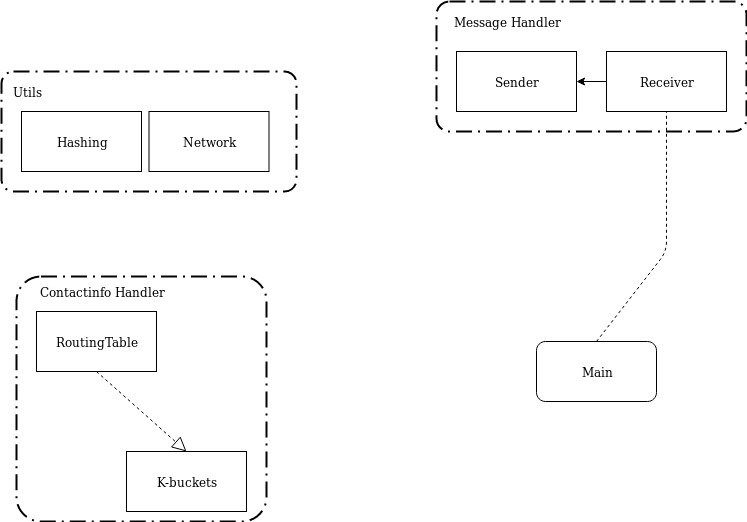
\includegraphics[width=\linewidth]{D7024E-architecture.jpg}
\caption{High-level architecture of a node in the kademlia implementation.}
\end{figure}

The main function starts the reciever listener as the 'busy-wait' loop so that the node does not terminate but awaits further instructions. The receiver then spawns new threads (goroutines) as needed to handle incoming instructions. The sender is used to send any messages to other nodes in the network. Utils handles any general functions such as hashing, a node getting its own IP, etc. While the routing table keeps records of a nodes k-buckets.

